% !TEX program = xelatex
\documentclass[a4paper,10pt]{article}

\makeatletter
\let\@expl@@@mark@update@singlecol@structures@@\relax
\makeatother

\usepackage[a4paper, left=0.95cm, right=0.95cm, top=0.85cm, bottom=0.92cm, footskip=0.52cm]{geometry}
\usepackage{fontspec}
\usepackage{amsmath, amssymb}
\usepackage{longtable, array, colortbl}
\usepackage[table]{xcolor}
\usepackage{fancyhdr}
\usepackage{tikz}
\usetikzlibrary{calc, angles, quotes, arrows.meta, decorations.markings}

% Cross-platform font discovery
\makeatletter
\newcommand{\NGSFindFonts}{%
  \IfFileExists{../../../fonts/KhmerOSsiemreap.ttf}{%
    \def\NGSUserPath{../../../fonts/}\def\NGSSysPath{../../../fonts/}%
  }{%
    \IfFileExists{../../../../fonts/KhmerOSsiemreap.ttf}{%
      \def\NGSUserPath{../../../../fonts/}\def\NGSSysPath{../../../../fonts/}%
    }{%
      \IfFileExists{fonts/KhmerOSsiemreap.ttf}{%
        \def\NGSUserPath{fonts/}\def\NGSSysPath{fonts/}%
      }{%
        \def\NGSUserPath{C:/Users/user/AppData/Local/Microsoft/Windows/Fonts/}%
        \def\NGSSysPath{C:/Windows/Fonts/}%
      }%
    }%
  }%
}
\NGSFindFonts
\makeatother

\XeTeXlinebreaklocale "km"
\XeTeXlinebreakskip = 0pt plus 1pt minus 0.1pt

\setmainfont[
  Path = {\NGSUserPath},
  Extension = .ttf,
  UprightFont = KhmerOSsiemreap,
  BoldFont = KhmerOSsiemreap,
  BoldFeatures = {FakeBold=1.8},
  ItalicFont = KhmerOSsiemreap,
  ItalicFeatures = {FakeSlant=0.25}
]{KhmerOSsiemreap}

\newfontfamily\muol[Path={\NGSUserPath}]{KhmerOSmuollight.ttf}
\newfontfamily\Tacteing[Path={\NGSUserPath}]{TACTENG.TTF}
\newfontfamily\enfont[Path={\NGSSysPath}, Scale=1.0]{times.ttf}
\newfontfamily\enbold[Path={\NGSSysPath}, Scale=1.0]{timesbd.ttf}
\newfontfamily\enital[Path={\NGSSysPath}, Scale=1.0]{timesi.ttf}
\newfontfamily\calibrifont[Path={\NGSSysPath}, Scale=0.95]{calibri.ttf}
\newfontfamily\symfont[Path={\NGSSysPath}, Scale=0.95]{cour.ttf}

\DeclareTextFontCommand{\en}{\enfont}
\newcommand{\enbf}[1]{{\enbold #1}}
\newcommand{\enit}[1]{{\enital #1}}
\newcommand{\khmflourish}{{\Tacteing\fontsize{17pt}{17pt}\selectfont 3}}
\newcommand{\wcirc}{{\symfont\char"25CB}}

\definecolor{headgray}{HTML}{E6E6E6}
\definecolor{stepgray}{HTML}{D4D4D4}
\definecolor{fiveecolor}{HTML}{8B0000}

\pagestyle{fancy}
\fancyhf{}
\renewcommand{\headrulewidth}{0pt}
\renewcommand{\footrulewidth}{0pt}
\fancyfoot[R]{{\calibrifont\fontsize{9.5pt}{11pt}\selectfont\thepage}}

\setlength{\parindent}{0pt}
\setlength{\LTpre}{2pt}
\setlength{\LTpost}{2pt}
\setlength{\tabcolsep}{4.5pt}
\newcolumntype{L}[1]{>{\raggedright\arraybackslash}p{#1}}

\newcommand{\fiveE}[2]{{\color{fiveecolor}\enbf{#1} \enit{(#2)}}}
\newcommand{\timenote}[1]{{\color{fiveecolor}\textit{#1}}}
\newcommand{\stepheader}[1]{%
  \rowcolor{stepgray}%
  \multicolumn{3}{|c|}{\rule[-4pt]{0pt}{15pt}{\muol\fontsize{10pt}{14pt}\selectfont #1}} \\*%
  \hline
}
\newcommand{\cfig}[1]{\begin{center}\vspace{-2pt}#1\vspace{-3pt}\end{center}}

\newcommand{\tri}[1]{\triangle #1}
\newcommand{\unit}[1]{\,\text{\en{#1}}}
\newcommand{\cnum}[1]{\tikz[baseline=-0.58ex]\node[circle, fill=black, text=white, inner sep=0.85pt, minimum size=1.95ex, font=\enbold\scriptsize]{#1};}

% Font-independent arc symbol above letters (\arc{AB})
\newcommand{\arc}[1]{\mbox{%
  \tikz[baseline=(arcX.base)]{%
    \node[inner sep=0pt, outer sep=0pt] (arcX) {$#1$};%
    \draw[black, line width=0.55pt] ($(arcX.north west)+(0.02,0.035)$) to[bend left=30] ($(arcX.north east)+(-0.02,0.035)$);%
  }%
}}

\newcommand{\rightbox}[4][0.20cm]{%
  \coordinate (rbA) at ($(#3)!#1!(#2)$);
  \coordinate (rbB) at ($(#3)!#1!(#4)$);
  \coordinate (rbC) at ($(rbA)+(#3)!#1!(#4)-(#3)$);
  \draw[black, line width=0.65pt] (rbA) -- (rbC) -- (rbB);
}

% ============================================================================
% ម៉ាក្រូរូបភាព TikZ ស-ខ្មៅ សមាមាត្រច្បាស់ (3.8 cm – 6.8 cm, អក្សរខ្មៅ 100%)
% ============================================================================

% ១. រូបបេសកកម្ម E1៖ រហាត់ទឹកស្ទឹងសែន (រង្វង់រួមផ្ចិតពីរជាន់ r1=1m, r2=2m ស្កាត់ដោយមុំ 60°)
\newcommand{\figEngageCIRCTwo}{%
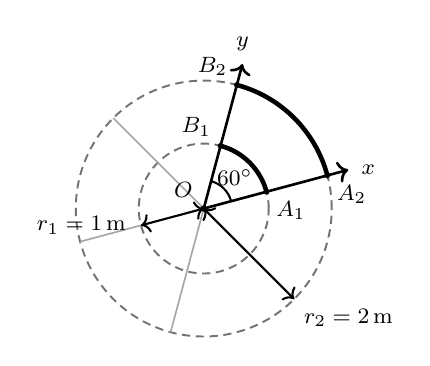
\begin{tikzpicture}[scale=0.50, every node/.style={font=\footnotesize, text=black}]
  \coordinate (O) at (0,0);
  \draw[black!55, line width=0.7pt, densely dashed] (O) circle (1.65);
  \draw[black!55, line width=0.7pt, densely dashed] (O) circle (3.25);
  \foreach \ang in {135,195,255,315} {
    \draw[black!35, line width=0.6pt] (O) -- (\ang:3.25);
  }
  \draw[black, line width=0.95pt, ->] (O) -- (15:3.80) node[right=1pt] {$x$};
  \draw[black, line width=0.95pt, ->] (O) -- (75:3.80) node[above=1pt] {$y$};
  \draw[black, line width=1.65pt] (15:1.65) arc (15:75:1.65);
  \draw[black, line width=1.65pt] (15:3.25) arc (15:75:3.25);
  \draw[black, line width=0.75pt] (15:0.72) arc (15:75:0.72);
  \node at (45:1.12) {$60^\circ$};
  % កាំ r1 និង r2 ដាក់នៅកាំផ្សេងមិនប៉ះអក្សរ A1, A2
  \draw[black, line width=0.75pt, <->] (O) -- (195:1.65);
  \node[left=2pt] at (195:1.65) {$r_1=1\unit{m}$};
  \draw[black, line width=0.75pt, <->] (O) -- (-45:3.25);
  \node[below right=0pt] at (-45:3.25) {$r_2=2\unit{m}$};
  \fill[black] (O) circle (2.3pt) (15:1.65) circle (2.1pt) (75:1.65) circle (2.1pt) (15:3.25) circle (2.1pt) (75:3.25) circle (2.1pt);
  \node[above left=0.5pt] at (O) {$O$};
  \node[below right=0pt] at (15:1.65) {$A_1$};
  \node[above left=0pt] at (75:1.65) {$B_1$};
  \node[below right=0pt] at (15:3.25) {$A_2$};
  \node[above left=0pt] at (75:3.25) {$B_2$};
\end{tikzpicture}}

% ២. រូប E2៖ មុំផ្ចិតលយ/ឆក (ឧទាហរណ៍ទី១) និងកាដ្រង់ទាំង ៤ (ឧទាហរណ៍ទី៣ ទំ.១៩៩)
\newcommand{\figExploreCIRCTwo}{%
\begin{tikzpicture}[scale=0.38, every node/.style={font=\scriptsize, text=black}]
  % ខាងឆ្វេង៖ មុំផ្ចិតលយ និងមុំផ្ចិតឆក (ទំ.១៩៩)
  \begin{scope}[shift={(0,0)}]
    \coordinate (O) at (3.0,2.9);
    \draw[black, line width=0.95pt] (O) circle (2.40);
    \draw[black, line width=1.55pt] ($(O)+(30:2.40)$) arc (30:135:2.40);
    \draw[black, line width=0.9pt, ->] (O) -- ($(O)+(30:3.05)$) node[right=0.5pt] {$y$};
    \draw[black, line width=0.9pt, ->] (O) -- ($(O)+(135:3.05)$) node[above left=0.5pt] {$x$};
    \draw[black, line width=0.75pt] ($(O)+(30:0.75)$) arc (30:135:0.75);
    \draw[black, line width=0.7pt, densely dashed] ($(O)+(135:0.55)$) arc (135:390:0.55);
    \fill[black] (O) circle (2.3pt) ($(O)+(135:2.40)$) circle (2.1pt) ($(O)+(30:2.40)$) circle (2.1pt) ($(O)+(-90:2.40)$) circle (2.0pt);
    \node[right=2pt] at ($(O)+(0,-0.15)$) {$O$};
    \node[above left=1pt] at ($(O)+(135:2.40)$) {$A$};
    \node[above right=1pt] at ($(O)+(30:2.40)$) {$B$};
    \node[below=1pt] at ($(O)+(-90:2.40)$) {$C$};
    \node[above=1pt] at ($(O)+(82.5:0.82)$) {មុំលយ};
    \node[below=2pt] at ($(O)+(-90:0.62)$) {មុំឆក};
    \node[align=center] at (3.0,-1.80) {ឧ.១៖ មុំលយស្កាត់ $\arc{AB}$\\មុំឆកស្កាត់ធ្នូធំ $\arc{ACB}$};
  \end{scope}
  % ខាងស្ដាំ៖ អង្កត់ផ្ចិតកែងគ្នា AB ⊥ CD បង្កើតបាន ៤ កាដ្រង់ (ទំ.១៩៩)
  \begin{scope}[shift={(9.3,0)}]
    \coordinate (O2) at (3.0,2.9);
    \draw[black, line width=1.0pt] (O2) circle (2.40);
    \draw[black!55, line width=0.7pt, densely dashed] (O2) circle (1.30);
    \draw[black, line width=0.9pt] ($(O2)+(-2.40,0)$) -- ($(O2)+(2.40,0)$);
    \draw[black, line width=0.9pt] ($(O2)+(0,-2.40)$) -- ($(O2)+(0,2.40)$);
    \rightbox[0.24cm]{$(O2)+(2.40,0)$}{O2}{$(O2)+(0,2.40)$}
    \fill[black] (O2) circle (2.3pt) ($(O2)+(-2.40,0)$) circle (2.1pt) ($(O2)+(2.40,0)$) circle (2.1pt) ($(O2)+(0,2.40)$) circle (2.1pt) ($(O2)+(0,-2.40)$) circle (2.1pt);
    \node[left=1pt] at ($(O2)+(-2.40,0)$) {$A$};
    \node[right=1pt] at ($(O2)+(2.40,0)$) {$B$};
    \node[above=1pt] at ($(O2)+(0,2.40)$) {$C$};
    \node[below=1pt] at ($(O2)+(0,-2.40)$) {$D$};
    \node[below left=0.5pt] at (O2) {$O$};
    \node at ($(O2)+(45:1.85)$) {$90^\circ$};
    \node at ($(O2)+(135:1.85)$) {$90^\circ$};
    \node[align=center] at (3.0,-1.80) {ឧ.៣៖ $AB \perp CD \Rightarrow 4$ កាដ្រង់\\($90^\circ$ ស្មើគ្នា ប្រវែងធ្នូតាម $r$)};
  \end{scope}
\end{tikzpicture}}

% ៣. រូប E4៖ លំហាត់គំរូទី១ (r=10dm, 36°) និងលំហាត់គំរូទី២ (r=15cm, 80°) (ទំ.១៩៩–២០០)
\newcommand{\figModelCIRCTwo}{%
\begin{tikzpicture}[scale=0.38, every node/.style={font=\scriptsize, text=black}]
  % លំហាត់គំរូទី១
  \begin{scope}[shift={(0,0)}]
    \coordinate (O) at (3.0,2.8);
    \draw[black, line width=0.95pt] (O) circle (2.35);
    \draw[black, line width=1.65pt] ($(O)+(10:2.35)$) arc (10:52:2.35);
    \draw[black, line width=0.9pt] (O) -- ($(O)+(10:2.35)$) (O) -- ($(O)+(52:2.35)$);
    \draw[black, line width=0.7pt] ($(O)+(10:0.95)$) arc (10:52:0.95);
    \fill[black] (O) circle (2.3pt) ($(O)+(10:2.35)$) circle (2.1pt) ($(O)+(52:2.35)$) circle (2.1pt);
    \node[left=1.5pt] at (O) {$O$};
    \node[right=1pt] at ($(O)+(10:2.35)$) {$A$};
    \node[above right=1pt] at ($(O)+(52:2.35)$) {$B$};
    \node at ($(O)+(31:1.52)$) {$36^\circ$};
    \node[below=2pt] at ($(O)+(10:1.25)$) {$10\unit{dm}$};
    \node[align=center] at (3.0,-1.55) {គំរូទី១ ($r=10\unit{dm}$)\\$\alpha=36^\circ \Rightarrow l = 6.28\unit{dm}$};
  \end{scope}
  % លំហាត់គំរូទី២
  \begin{scope}[shift={(9.3,0)}]
    \coordinate (O2) at (3.0,2.8);
    \draw[black, line width=0.95pt] (O2) circle (2.35);
    \draw[black, line width=1.65pt] ($(O2)+(10:2.35)$) arc (10:90:2.35);
    \draw[black, line width=0.9pt] (O2) -- ($(O2)+(10:2.35)$) (O2) -- ($(O2)+(90:2.35)$);
    \draw[black, line width=0.7pt] ($(O2)+(10:0.80)$) arc (10:90:0.80);
    \fill[black] (O2) circle (2.3pt) ($(O2)+(10:2.35)$) circle (2.1pt) ($(O2)+(90:2.35)$) circle (2.1pt);
    \node[below left=1pt] at (O2) {$O$};
    \node[right=1pt] at ($(O2)+(10:2.35)$) {$A$};
    \node[above=1pt] at ($(O2)+(90:2.35)$) {$B$};
    \node at ($(O2)+(48:1.25)$) {$80^\circ$};
    \node[below=2pt] at ($(O2)+(10:1.25)$) {$15\unit{cm}$};
    \node[align=center] at (3.0,-1.55) {គំរូទី២ ($r=15\unit{cm}$)\\$\arc{AB}=80^\circ \Rightarrow l \approx 20.93\unit{cm}$};
  \end{scope}
\end{tikzpicture}}

% ៤. រូប E5៖ ប្រតិបត្តិ ទំ.២០០ (ធ្នូមិនប៉ុនគ្នា) និងលំហាត់ទី១ ទំ.២០៤ (∠AOB = 25°)
\newcommand{\figPracticeCIRCTwo}{%
\begin{tikzpicture}[scale=0.38, every node/.style={font=\scriptsize, text=black}]
  % ប្រតិបត្តិ ទំ.២០០
  \begin{scope}[shift={(0,0)}]
    \coordinate (O) at (3.0,2.8);
    \draw[black, line width=0.95pt] (O) circle (2.35);
    \draw[black, line width=1.6pt] ($(O)+(135:2.35)$) arc (135:175:2.35);
    \draw[black, line width=1.6pt] ($(O)+(-35:2.35)$) arc (-35:50:2.35);
    \draw[black, line width=0.85pt] (O)--($(O)+(135:2.35)$) (O)--($(O)+(175:2.35)$) (O)--($(O)+(-35:2.35)$) (O)--($(O)+(50:2.35)$);
    \fill[black] (O) circle (2.2pt) ($(O)+(135:2.35)$) circle (2pt) ($(O)+(175:2.35)$) circle (2pt) ($(O)+(-35:2.35)$) circle (2pt) ($(O)+(50:2.35)$) circle (2pt);
    \node[below=1pt] at (O) {$O$};
    \node[above left=0.5pt] at ($(O)+(135:2.35)$) {$A$};
    \node[left=0.5pt] at ($(O)+(175:2.35)$) {$B$};
    \node[above right=0.5pt] at ($(O)+(50:2.35)$) {$C$};
    \node[below right=0.5pt] at ($(O)+(-35:2.35)$) {$D$};
    \node[align=center] at (3.0,-1.55) {ប្រតិបត្តិ៖ $\arc{AB} < \arc{CD}$\\$\Rightarrow \angle AOB < \angle COD$};
  \end{scope}
  % លំហាត់ទី១ ទំ.២០៤
  \begin{scope}[shift={(9.3,0)}]
    \coordinate (O2) at (3.0,2.8);
    \draw[black, line width=0.95pt] (O2) circle (2.35);
    \draw[black, line width=1.6pt] ($(O2)+(-16:2.35)$) arc (-16:18:2.35);
    \draw[black, line width=0.85pt] (O2)--($(O2)+(-16:2.35)$) (O2)--($(O2)+(18:2.35)$);
    \draw[black, line width=0.7pt] ($(O2)+(-16:0.95)$) arc (-16:18:0.95);
    \fill[black] (O2) circle (2.2pt) ($(O2)+(-16:2.35)$) circle (2pt) ($(O2)+(18:2.35)$) circle (2pt);
    \node[left=2pt] at (O2) {$O$};
    \node[above right=0.5pt] at ($(O2)+(18:2.35)$) {$A$};
    \node[below right=0.5pt] at ($(O2)+(-16:2.35)$) {$B$};
    \node at ($(O2)+(1:1.52)$) {$25^\circ$};
    \node[align=center] at (3.0,-1.55) {លំហាត់ទី១៖ $\angle AOB = 25^\circ$\\$\Rightarrow \arc{AB} = 25^\circ$};
  \end{scope}
\end{tikzpicture}}

\begin{document}
\fontsize{10pt}{15.0pt}\selectfont

% ==================== ក្បាលរដ្ឋបាលផ្លូវការ ====================
{\centering
  {\muol\fontsize{11pt}{16pt}\selectfont ព្រះរាជាណាចក្រកម្ពុជា}\\[2pt]
  {\muol\fontsize{11pt}{16pt}\selectfont ជាតិ សាសនា ព្រះមហាក្សត្រ}\\[-2pt]
  \khmflourish\par
}
\vspace{-4pt}
{\muol\fontsize{10pt}{15.2pt}\selectfont
មន្ទីរអប់រំ យុវជន និងកីឡា ខេត្តកំពង់ធំ\\
ការិយាល័យអប់រំ យុវជន និងកីឡា ស្រុកកំពង់ស្វាយ\\
អនុវិទ្យាល័យព្រះក្រសាំង\par}

\vspace{2pt}
{\centering{\muol\fontsize{12pt}{18pt}\selectfont កិច្ចតែងការបង្រៀន}\par}
\vspace{2pt}

{\fontsize{10pt}{15.0pt}\selectfont
\hspace*{3.7cm}%
\begin{tabular}{@{}l l l l@{}}
  - & មុខវិជ្ជា & : & គណិតវិទ្យា ថ្នាក់ទី៨ \\
  - & ចំណងជើងមេរៀន & : & មេរៀនទី១៥ រង្វង់ \\
  - & ចំណងជើងរង & : & ២. មុំផ្ចិត និងធ្នូ — រង្វាស់ធ្នូ និងប្រវែងធ្នូ (ទំព័រ ១៩៩--២០០) \\
  - & រយៈពេល & : & ១ ម៉ោងសិក្សា (៥០ នាទី) \\
  - & បង្រៀនដោយ & : & ហុក ប៊ុនថែន \\
  - & កាលបរិច្ឆេទ & : & ថ្ងៃសៅរ៍ ទី១៩ ខែធ្នូ ឆ្នាំ២០២៦ \\
\end{tabular}

\vspace{1pt}

% -------------------- I. វត្ថុបំណង --------------------
\textbf{I.} {\muol វត្ថុបំណង}\\[1pt]
\hspace*{0.55cm}%
\begin{tabular}{@{}l l L{14.2cm}@{}}
  \wcirc \hspace{0.25cm} វិជ្ជាសម្បទា & : & សិស្សប្រាប់និយមន័យមុំផ្ចិត (មុំលយ និងមុំឆក) ធ្នូស្កាត់ដោយមុំផ្ចិត កាដ្រង់ ($90^\circ$) ទំនាក់ទំនងរវាងមុំផ្ចិតនិងរង្វាស់ធ្នូគិតជាដឺក្រេ ព្រមទាំងរូបមន្តប្រវែងធ្នូ $l = \frac{2\pi r \times \alpha}{360^\circ}$ បានត្រឹមត្រូវ ។ \\
  \wcirc \hspace{0.25cm} បំណិនសម្បទា & : & សិស្សញែកដាច់ពីគ្នារវាងរង្វាស់ធ្នូគិតជាដឺក្រេនិងប្រវែងធ្នូគិតជាឯកតាប្រវែង និងគណនាប្រវែងធ្នូនៃរង្វង់តាមសមាមាត្រធៀបនឹងបរិមាត្ររង្វង់លើសន្លឹកកិច្ចការបានត្រឹមត្រូវ ។ \\
  \wcirc \hspace{0.25cm} ចរិយាសម្បទា & : & សិស្សមានភាពម៉ត់ចត់ក្នុងការប្រើប្រាស់ខ្នាតដឺក្រេនិងខ្នាតប្រវែង សហការពិភាក្សាដៃគូ និងឱ្យតម្លៃលើការគណនាប្រវែងធ្នូក្នុងសិប្បកម្មរហាត់ទឹកនិងជីវភាពពិត ។ \\
\end{tabular}

\vspace{1pt}

% -------------------- II. សម្ភារៈឧបទេស --------------------
\textbf{II.} {\muol សម្ភារៈឧបទេស}\\[1pt]
\hspace*{0.55cm}\parbox[t]{18.2cm}{$\bullet$ \hspace{0.25cm} សម្រាប់គ្រូ៖ សៀវភៅសិក្សាគោលគណិតវិទ្យាថ្នាក់ទី៨ (ទំ.១៩៩--២០០ និង ២០៤) ក្ដារខៀន ដីស ដែកឈាន និងរ៉ាប់ព័រទ័រក្ដារខៀន (គ្មានស្លាយ \en{LCD}) ។\\
$\bullet$ \hspace{0.25cm} សម្រាប់សិស្ស៖ សន្លឹកកិច្ចការសិស្ស ស-ខ្មៅ (\en{Worksheet\_CIRC2} ២ ទំព័រពេញ) សៀវភៅគោល រ៉ាប់ព័រទ័រវាស់មុំ និងបន្ទាត់ក្រិត ។}

\vspace{1pt}

% -------------------- III. វិធីសាស្រ្តបង្រៀន --------------------
\textbf{III.} {\muol វិធីសាស្រ្តបង្រៀន}\\[1pt]
\hspace*{0.45cm}%
\begin{tabular}{@{}l l L{14.85cm}@{}}
  $\bullet$ \hspace{0.25cm} គោលវិធី & : & សិស្សមជ្ឈមណ្ឌល (បង្រៀនដោយមិនប្រើស្លាយ \en{LCD} យកសន្លឹកកិច្ចការតារាងសមាមាត្រជាគោល) \\
  $\bullet$ \hspace{0.25cm} យុទ្ធវិធីបង្រៀន & : & គំរូ \en{5Es} រួមផ្សំតំណាង \en{CPA} លើរង្វង់រួមផ្ចិតពីរជាន់ (បំបែកការច្រឡំដឺក្រេធ្នូ និងប្រវែងធ្នូ) \\
\end{tabular}
}

\vspace{1pt}

% -------------------- IV. ដំណើរការបង្រៀន --------------------
\textbf{IV.} {\muol ដំណើរការបង្រៀន}

\vspace{1pt}

\renewcommand{\arraystretch}{1.15}
\begin{longtable}{|L{5.50cm}|L{7.90cm}|L{4.80cm}|}
\hline
\rowcolor{headgray}
\multicolumn{1}{|c|}{\muol សកម្មភាពគ្រូ} &
\multicolumn{1}{c|}{\muol ខ្លឹមសារមេរៀន} &
\multicolumn{1}{c|}{\muol សកម្មភាពសិស្ស} \\
\hline
\endfirsthead

\hline
\rowcolor{headgray}
\multicolumn{1}{|c|}{\muol សកម្មភាពគ្រូ} &
\multicolumn{1}{c|}{\muol ខ្លឹមសារមេរៀន} &
\multicolumn{1}{c|}{\muol សកម្មភាពសិស្ស} \\
\hline
\endhead

\hline
\endfoot

\hline
\endlastfoot

% ==================== ជំហានទី១ (2min) ====================
\stepheader{ជំហានទី១ ៖ រដ្ឋបាលថ្នាក់ (២ នាទី)}
$\bullet$ ពិនិត្យអវត្តមាន សណ្ដាប់ធ្នាប់ និងការត្រៀមរ៉ាប់ព័រទ័រវាស់មុំរបស់សិស្ស\par\vspace{1pt}
$\bullet$ ចែកសន្លឹកកិច្ចការ \en{Worksheet\_CIRC2} (១ សន្លឹកសងខាង) ដល់សិស្សគ្រប់គ្នា
&
$\bullet$ ពិនិត្យវត្តមាន វិន័យ និងសម្ភារៈសិក្សា (សន្លឹកកិច្ចការ រ៉ាប់ព័រទ័រ និងបន្ទាត់ក្រិត)
&
$\circ$ ប្រធានថ្នាក់រាយការណ៍អវត្តមាន\par\vspace{1pt}
$\circ$ ទទួលសន្លឹកកិច្ចការ និងសរសេរឈ្មោះ \\[3pt]
\hline

% ==================== ជំហានទី២ (9min: ≤3 + 3 + E1 3) ====================
\stepheader{ជំហានទី២ ៖ កែកិច្ចការផ្ទះ រំលឹកមេរៀនចាស់ និងភ្ជាប់មេរៀនថ្មី (៩ នាទី)}
\timenote{(កែកិច្ចការផ្ទះ $\le 3\unit{min}$)}\par\vspace{1pt}
$\bullet$ ហៅសិស្ស ២ នាក់ឡើងបង្ហាញគន្លឹះសម្រាយបញ្ជាក់លំហាត់ទី៦ និងទី៧ (ទំ.២០៤) យ៉ាងខ្លីលើក្ដារខៀន
&
\textbf{កំណែកិច្ចការផ្ទះ (ទំ.២០៤)៖}\par\vspace{1pt}
១. \textbf{លំហាត់ទី៦៖} អង្កត់មធ្យម $\tri{ABC}$ សម័ង្សឱ្យ $JI = JK = JB = JC = \frac{1}{2}AB \Rightarrow B,I,K,C \in C(J, JB)$ ។\par\vspace{1pt}
២. \textbf{លំហាត់ទី៧៖} $AC \perp BD \Rightarrow MNRS$ ជាចតុកោណកែងមានអង្កត់ទ្រូង $MR = NS$ កាត់គ្នាត្រង់ $O \Rightarrow OM=ON=OR=OS$ ។
&
$\circ$ ផ្ទៀងផ្ទាត់គន្លឹះសម្រាយបញ្ជាក់ និងកែតម្រូវចូលសៀវភៅ \\[3pt]

\timenote{(រំលឹកមេរៀនទាក់ទង $3\unit{min}$)}\par\vspace{1pt}
$\bullet$ សួររំលឹករូបមន្តបរិមាត្ររង្វង់៖ «តើបរិមាត្ររង្វង់កាំ $r$ ស្មើប៉ុន្មាន?»
&
\textbf{រំលឹកបរិមាត្ររង្វង់ និងមុំពេញ៖}\par\vspace{1pt}
$\bullet$ បរិមាត្ររង្វង់កាំ $r$ គឺ $P = 2\pi r = \pi d$ (ដែល $\pi \approx 3.14$) ។
&
$\circ$ ឆ្លើយរំលឹករូបមន្តបរិមាត្ររង្វង់ $P = 2\pi r$ \\[3pt]

$\bullet$ សួរបន្តអំពីរង្វាស់មុំពេញមួយជុំផ្ចិត $O$ និងកន្លះរង្វង់
&
$\bullet$ មុំពេញជុំវិញផ្ចិត $O$ មានរង្វាស់ស្មើនឹង $360^\circ$ (កន្លះរង្វង់ស្មើនឹង $180^\circ$) ។
&
$\circ$ ឆ្លើយរំលឹករង្វាស់មុំពេញ $360^\circ$ និងកន្លះរង្វង់ $180^\circ$ \\[3pt]

\fiveE{E1 - Engage}{3 min}\par\vspace{1pt}
$\bullet$ ឱ្យសិស្សពិនិត្យ \textbf{ផ្នែកទី១} លើសន្លឹកកិច្ចការ៖ ជាងធ្វើ \textbf{រហាត់ទឹកស្ទឹងសែន} ពត់ខ្នងឫស្សីរួមផ្ចិតពីរជាន់ ($r_1 = 1\unit{m}$ និង $r_2 = 2\unit{m}$) ចន្លោះកាំពីរធ្វើមុំ $60^\circ$
&
\textbf{បេសកកម្ម E1៖ រហាត់ទឹកស្ទឹងសែនពីរជាន់ ($r_1=1\unit{m},\; r_2=2\unit{m}$)}\par\vspace{1pt}
$\bullet$ សំណួរបំផុសពីរ៖ (១) តើធ្នូក្នុង $\arc{A_1B_1}$ និងធ្នូក្រៅ $\arc{A_2B_2}$ មាន \textbf{រង្វាស់ដឺក្រេ} ស្មើគ្នាឬទេ? (២) តើបន្ទះឫស្សីទាំងពីរមាន \textbf{ប្រវែងម៉ែត្រ} ស្មើគ្នាឬទេ? (ទុកផ្ទៀងនៅ E5)
&
$\circ$ សង្កេតរូបរហាត់ទឹក និងគូសធីកទស្សន៍ទាយទាំង ២ សំណួរលើសន្លឹកកិច្ចការ \\[3pt]

&
\cfig{\figEngageCIRCTwo}
& \\[3pt]
\hline

% ==================== ជំហានទី៣ (17min: E2 11 + E3 6) ====================
\stepheader{ជំហានទី៣ ៖ រុករកមុំផ្ចិត រង្វាស់ធ្នូ និងតារាងសមាមាត្រប្រវែងធ្នូ (១៧ នាទី)}
\fiveE{E2 - Explore}{11 min}\par\vspace{1pt}
$\bullet$ ឱ្យដៃគូសិស្សពិនិត្យរូបក្នុង \textbf{ផ្នែកទី២ (ក)} (ឧទាហរណ៍ទី១--៣ ទំ.១៩៩) ប្រើរ៉ាប់ព័រទ័រវាស់មុំផ្ចិតលយ $\angle xOy$ និងគណនាមុំឆក
&
\textbf{សកម្មភាពទី១៖ មុំផ្ចិត ធ្នូ និងកាដ្រង់ (ទំ.១៩៩)}\par\vspace{1pt}
$\bullet$ កន្លះបន្ទាត់ $Ox, Oy$ កាត់រង្វង់ត្រង់ $A, B$ បង្កើតបាន \textbf{មុំផ្ចិតពីរ}៖ \textbf{មុំលយ} (ស្កាត់ធ្នូតូច $\arc{AB}$) និង \textbf{មុំឆក} (ស្កាត់ធ្នូធំ $\arc{ACB}$) ដោយ $\text{មុំលយ} + \text{មុំឆក} = 360^\circ$ ។
&
$\circ$ វាស់មុំលយ និងគណនាមុំឆកលើសន្លឹកកិច្ចការ \\[3pt]

$\bullet$ ឱ្យដៃគូពិនិត្យករណីអង្កត់ផ្ចិតពីរកែងគ្នា $AB \perp CD$ (ឧទាហរណ៍ទី៣)
&
$\bullet$ បើអង្កត់ផ្ចិត $AB \perp CD$ នោះមុំផ្ចិតទាំងបួនស្មើគ្នា ($90^\circ$) ចែករង្វង់ជា $4$ \textbf{កាដ្រង់} ប៉ុនៗគ្នា ។
&
$\circ$ កត់សម្គាល់និយមន័យកាដ្រង់ ($90^\circ$) លើសន្លឹកកិច្ចការ \\[3pt]

$\bullet$ ដឹកនាំដៃគូសិស្សបំពេញ \textbf{តារាងសមាមាត្រប្រវែងធ្នូ} ក្នុង \textbf{ផ្នែកទី២ (ខ)} ដោយប្រៀបធៀបធ្នូ $360^\circ, 180^\circ, 90^\circ, 1^\circ$ និង $\alpha^\circ$
&
\textbf{សកម្មភាពទី២៖ តារាងសមាមាត្របំបែកការច្រឡំដឺក្រេ និងប្រវែងធ្នូ}\par\vspace{1pt}
-- មួយជុំរង្វង់ ($360^\circ$) មានប្រវែងស្មើបរិមាត្រ $P = 2\pi r$ $\Rightarrow$ ធ្នូ $1^\circ$ មានប្រវែង $\frac{P}{360^\circ} = \frac{2\pi r}{360^\circ}$ ។
&
$\circ$ បំពេញប្រភាគនៃបរិមាត្រសម្រាប់ $180^\circ, 90^\circ$ និង $1^\circ$ \\[3pt]

$\bullet$ ឱ្យសិស្សទាញរូបមន្តប្រវែងធ្នូទូទៅសម្រាប់មុំផ្ចិត $\alpha^\circ$ និងប្រៀបធៀបឥទ្ធិពលនៃកាំ $r$
&
-- ធ្នូស្កាត់ដោយមុំផ្ចិត $\alpha^\circ$ មាន \textbf{រង្វាស់ដឺក្រេស្មើ $\alpha^\circ$} (មិនអាស្រ័យលើកាំ $r$ ទេ) តែមាន \textbf{ប្រវែងធ្នូ} $l = \frac{P \times \alpha}{360^\circ} = \frac{2\pi r \times \alpha}{360^\circ}$ (ប្រែប្រួលតាមកាំ $r$!) ។
&
$\circ$ ទាញរូបមន្ត $l = \frac{2\pi r \times \alpha}{360^\circ}$ និងពិភាក្សាដៃគូ \\[3pt]

&
\cfig{\figExploreCIRCTwo}
& \\[3pt]

\fiveE{E3 - Explain}{6 min}\par\vspace{1pt}
$\bullet$ សំយោគទ្រឹស្ដីបទធ្នូប៉ុនគ្នា និងធ្នូមិនប៉ុនគ្នា តាមអត្ថបទសៀវភៅគោល (ទំ.១៩៩)
&
\textbf{បញ្ញត្តិ ទ្រឹស្ដីបទ និងរូបមន្តប្រវែងធ្នូ (ទំ.១៩៩)៖}\par\vspace{1pt}
$\bullet$ \textbf{ជាទូទៅ (ក្នុងរង្វង់តែមួយ ឬរង្វង់ពីរប៉ុនគ្នា)៖}\par
១. ធ្នូពីរប៉ុនគ្នា ស្កាត់ដោយមុំផ្ចិតពីរប៉ុនគ្នា និងច្រាសមកវិញ ($\arc{AB} = \arc{DE} \Leftrightarrow \angle AOB = \angle DOE$) ។
&
$\circ$ បំពេញលក្ខណៈទី១ ក្នុង \textbf{ផ្នែកទី៣} នៃសន្លឹកកិច្ចការ \\[3pt]

$\bullet$ សួរបញ្ជាក់ករណីធ្នូពីរមិនប៉ុនគ្នា និងសម្គាល់ធ្នូ $1^\circ$
&
២. ធ្នូពីរមិនប៉ុនគ្នា ធ្នូធំជាងស្កាត់ដោយមុំផ្ចិតធំជាង ($\arc{CD} > \arc{AB} \Leftrightarrow \angle COD > \angle AOB$) ។\par\vspace{1pt}
$\bullet$ \textbf{សម្គាល់៖} ធ្នូ $1^\circ$ ជាធ្នូដែលស្កាត់ដោយមុំផ្ចិតមានរង្វាស់ស្មើនឹង $1^\circ$ ។
&
$\circ$ បំពេញលក្ខណៈទី២ និងឆ្លើយសំណួរពិត/មិនពិត \\[3pt]

$\bullet$ ឱ្យសិស្សសង្ខេបតារាងប្រៀបធៀប \textbf{រង្វាស់ធ្នូគិតជាដឺក្រេ} និង \textbf{ប្រវែងធ្នូ $l$} ដើម្បីកុំឱ្យច្រឡំខ្នាត
&
{\fontsize{8.8pt}{12pt}\selectfont\renewcommand{\arraystretch}{1.16}
\begin{tabular}{|L{2.25cm}|L{2.45cm}|L{2.45cm}|}
\hline
\cellcolor{headgray}\centering\textbf{លក្ខណៈប្រៀបធៀប} &
\cellcolor{headgray}\centering\textbf{រង្វាស់ធ្នូ (ដឺក្រេ)} &
\cellcolor{headgray}\centering\arraybackslash\textbf{ប្រវែងធ្នូ ($l$)} \\[2pt]
\hline
រូបមន្តគណនា & $\text{រង្វាស់ }\arc{AB} = \angle AOB = \alpha^\circ$ & $l = \dfrac{2\pi r \times \alpha}{360^\circ}$ \\[3pt]
\hline
ខ្នាតរង្វាស់ & ដឺក្រេ ($^\circ$) & $\unit{mm},\unit{cm},\unit{dm},\unit{m}$ \\[1.5pt]
\hline
ឥទ្ធិពលនៃកាំ $r$ & \textbf{មិនអាស្រ័យលើ $r$} & \textbf{សមាមាត្រនឹង $r$} \\[1.5pt]
\hline
\end{tabular}}
&
$\circ$ កត់ត្រារូបមន្ត និងតារាងញែកដឺក្រេធ្នូ ទល់នឹងប្រវែងធ្នូ $l$ \\[3pt]
\hline

% ==================== ជំហានទី៤ (20min: E4 10 + E5 10) ====================
\stepheader{ជំហានទី៤ ៖ ពង្រឹងចំណេះដឹងតាមលំហាត់គំរូ និងវាយតម្លៃ (២០ នាទី)}
\fiveE{E4 - Elaborate}{10 min}\par\vspace{1pt}
$\bullet$ ដឹកនាំសិស្សដោះស្រាយ \textbf{លំហាត់គំរូទី១ (ទំ.១៩៩--២០០)} លើ \textbf{ផ្នែកទី៤} និងបញ្ជាក់ភាពលម្អៀងនៃការបង្គត់តម្លៃ $\pi$
&
\textbf{១. លំហាត់គំរូទី១ (ទំ.១៩៩--២០០)៖} រង្វង់កាំ $r = 10\unit{dm}$ មានធ្នូស្កាត់ដោយមុំផ្ចិត $\alpha = 36^\circ$ ។ រកប្រវែងធ្នូគិតជា $\unit{dm}$ ។\par\vspace{1pt}
-- បរិមាត្ររង្វង់ ($360^\circ$)៖ យក $\pi \approx 3.14 \Rightarrow P = 2\pi r = 2 \times 3.14 \times 10 = 62.8\unit{dm}$ ។
&
$\circ$ គណនាបរិមាត្ររង្វង់ $P = 62.8\unit{dm}$ លើសន្លឹកកិច្ចការ \\[3pt]

$\bullet$ ឱ្យសិស្សគណនាប្រវែងធ្នូ $36^\circ$ និងផ្ទៀងផ្ទាត់តួលេខក្នុងសៀវភៅគោល
&
-- ប្រវែងធ្នូ $36^\circ$៖ $l = \dfrac{62.8 \times 36^\circ}{360^\circ} = \mathbf{6.28\unit{dm}}$ \textit{(សម្គាល់៖ បើយក $\pi \approx 3.1416$ បាន $P = 62.832\unit{dm},\; l \approx 6.283\unit{dm}$)} ។
&
$\circ$ គណនា $l = 6.28\unit{dm}$ និងកត់សម្គាល់ការបង្គត់ $\pi$ \\[3pt]

$\bullet$ ឱ្យសិស្សបន្តដោះស្រាយ \textbf{លំហាត់គំរូទី២ (ទំ.២០០)} ដោយរក្សាខ្នាត $\unit{cm}$ ឱ្យត្រឹមត្រូវ
&
\textbf{២. លំហាត់គំរូទី២ (ទំ.២០០)៖} រង្វង់កាំ $r = 15\unit{cm}$ ($\pi = 3.14$) មានធ្នូ $\arc{AB} = 80^\circ$ ។ រកប្រវែងធ្នូ $\arc{AB}$ ។\par\vspace{1pt}
-- បរិមាត្ររង្វង់៖ $P = 2 \times 3.14 \times 15 = 94.2\unit{cm}$ ។\par\vspace{1pt}
-- ប្រវែងធ្នូ $80^\circ$៖ $l = \dfrac{94.2 \times 80^\circ}{360^\circ} = \dfrac{94.2 \times 2}{9} = \dfrac{62.8}{3} \approx \mathbf{20.93\unit{cm}}$ ។
&
$\circ$ បំពេញជំហានគណនា $P = 94.2\unit{cm}$ និង $l \approx 20.93\unit{cm}$ ផ្ទៀងជាមួយដៃគូ \\[3pt]

&
\cfig{\figModelCIRCTwo}
& \\[3pt]

\fiveE{E5 - Evaluate}{10 min}\par\vspace{1pt}
$\bullet$ ឱ្យសិស្សធ្វើ \textbf{ប្រតិបត្តិ (ទំ.២០០)} និង \textbf{លំហាត់ទី១ (ទំ.២០៤)} ដោយខ្លួនឯងលើ \textbf{ផ្នែកទី៥} នៃសន្លឹកកិច្ចការ
&
\textbf{១. ប្រតិបត្តិ (ទំ.២០០)៖} ក្នុង $C(O,r)$ ធ្នូតូចពីរមិនប៉ុនគ្នា $\arc{AB} < \arc{CD}$ $\Rightarrow$ ប្រៀបធៀបមុំផ្ចិតបាន $\mathbf{\angle AOB < \angle COD}$ (ព្រោះធ្នូតូចជាងស្កាត់ដោយមុំផ្ចិតតូចជាង) ។\par\vspace{1pt}
\textbf{២. លំហាត់ទី១ (ទំ.២០៤)៖} មុំផ្ចិត $\angle AOB = 25^\circ \Rightarrow$ រង្វាស់ធ្នូតូច $\arc{AB} = \mathbf{25^\circ}$ (ឯធ្នូធំមានរង្វាស់ $360^\circ - 25^\circ = \mathbf{335^\circ}$) ។
&
$\circ$ សរសេរការប្រៀបធៀបមុំផ្ចិត និងគណនារង្វាស់ធ្នូតូច/ធ្នូធំដោយខ្លួនឯង \\[3pt]

&
\cfig{\figPracticeCIRCTwo}
& \\[3pt]

$\bullet$ ពិនិត្យចម្លើយបិទបេសកកម្មរហាត់ទឹក E1 និងធ្វើតេស្តរហ័ស ៦០ វិនាទី (\en{Exit Check})
&
$\bullet$ \textbf{បិទបេសកកម្ម E1៖} (១) ធ្នូក្នុងនិងធ្នូក្រៅមាន \textbf{រង្វាស់ដឺក្រេស្មើគ្នា $60^\circ$} ។ (២) ប្រវែងឫស្សី \textbf{មិនស្មើគ្នាទេ}៖ $l_1 = \frac{2\times 3.14\times 1\times 60^\circ}{360^\circ} \approx 1.05\unit{m}$ ឯ $l_2 \approx 2.09\unit{m} = 2l_1$!\par\vspace{1pt}
$\bullet$ \textbf{Exit Check៖} រង្វង់រួមផ្ចិតពីរមានកាំ $r_1 = 5\unit{cm}$ និង $r_2 = 10\unit{cm}$ ស្កាត់ដោយមុំផ្ចិត $72^\circ$ ៖ \textbf{A. ដឺក្រេស្មើគ្នា $72^\circ$ តែ $l_2 = 2l_1$ (ត្រូវ)} $\;\vert\;$ B. $l_1 = l_2$ $\;\vert\;$ C. ធ្នូក្រៅ $144^\circ$ ។
&
$\circ$ គណនាបិទបេសកកម្មរហាត់ទឹក និងលើកម្រាមដៃទី១ ជ្រើសចម្លើយ \textbf{A} \\[3pt]
\hline

% ==================== ជំហានទី៥ (≤2min) ====================
\stepheader{ជំហានទី៥ ៖ កិច្ចការផ្ទះ និងបណ្ដាំផ្ញើ ($\le$ ២ នាទី)}
\timenote{(ចំណាយពេល $\le 2\unit{min}$)}\par\vspace{1pt}
$\bullet$ ដាក់កិច្ចការផ្ទះពង្រីកពីលំហាត់ទី១ (ទំ.២០៤)\par\vspace{1pt}
$\bullet$ ផ្ដាំផ្ញើឱ្យអានមុន ចំណុច \textbf{២.១ ធ្នូ និងអង្កត់ធ្នូ} (ទំ.២០០--២០១) និងយកបន្ទាត់ក្រិត ដែកឈានមកម៉ោងក្រោយ
&
\textbf{កិច្ចការផ្ទះ (ពង្រឹងមុំផ្ចិត និងប្រវែងធ្នូ — ភ្ជាប់ទំ.២០៤)៖}\par\vspace{1pt}
១. ក្នុងរង្វង់ $C(O, 18\unit{cm})$ គេមានមុំផ្ចិត $\angle AOB = 25^\circ$ និង $\angle COD = 120^\circ$ ។ ចូរគណនារង្វាស់ដឺក្រេនៃធ្នូធំ $\arc{ACB}$ និងប្រវែងធ្នូតូចទាំងពីរ ($\pi \approx 3.14$) ។\par\vspace{1pt}
២. \textbf{ចំណោទច្រាស៖} ធ្នូ $\arc{MN}$ មួយនៅលើរង្វង់កាំ $r = 15\unit{cm}$ មានប្រវែង $l = 15.7\unit{cm}$ ($\pi \approx 3.14$) ។ ចូរគណនារង្វាស់មុំផ្ចិត $\angle MON$ គិតជាដឺក្រេ ។
&
$\circ$ កត់ត្រាកិច្ចការផ្ទះចូលសៀវភៅ និងត្រៀមអានចំណុច ២.១ មុន\par\vspace{1pt}
$\circ$ ទទួលបណ្ដាំផ្ញើ និងជម្រាបលាគ្រូ \\[3pt]
\end{longtable}

% -------------------- កាលបរិច្ឆេទ និងហត្ថលេខា --------------------
\vspace{8pt}
\hfill
\begin{minipage}{9.8cm}
  {\centering
    ថ្ងៃសៅរ៍ ១០កើត ខែមិគសិរ ឆ្នាំមមី អដ្ឋស័ក ពុទ្ធសករាជ ២៥៧០\\[2pt]
    ព្រះក្រសាំង, ថ្ងៃទី១៩ ខែធ្នូ ឆ្នាំ២០២៦\\[3pt]
    {\muol គ្រូបង្រៀន}\par}
  \vspace{26pt}
  \hfill{\muol ហុក ប៊ុនថែន}\hspace*{1.4cm}
\end{minipage}

\end{document}
